\subsubsection{Navigation}
Our original approach was to search the panel by using long range
laser sensor. However, it was found to be difficult to detect the panel at a
distance because of the low density of points provided by the sensor.
Therefore, we use a second approach where the robot navigates around
the arena and searches for the panel using the point cloud data from its
stereo camera. Initially, if the panel is not visible within the
robot's field of view, meaning that the panel is either out of range
of the camera or is in another direction, the robot will navigate
around the arena to search for the panel. Then, when the panel is in
the sensing range of the stereo camera, the robot recognizes the panel
by finding the cluster of points in the point cloud that sits
approximately 1 meter above the ground (Fig.\ref{fig:
  task2_panel-recognition}) and approaches the panel. Finally, the
robot circles around the panel to recognize its front side, then move
to position itself in front of the panel.

\begin{figure}[htb]
  \begin{center}
    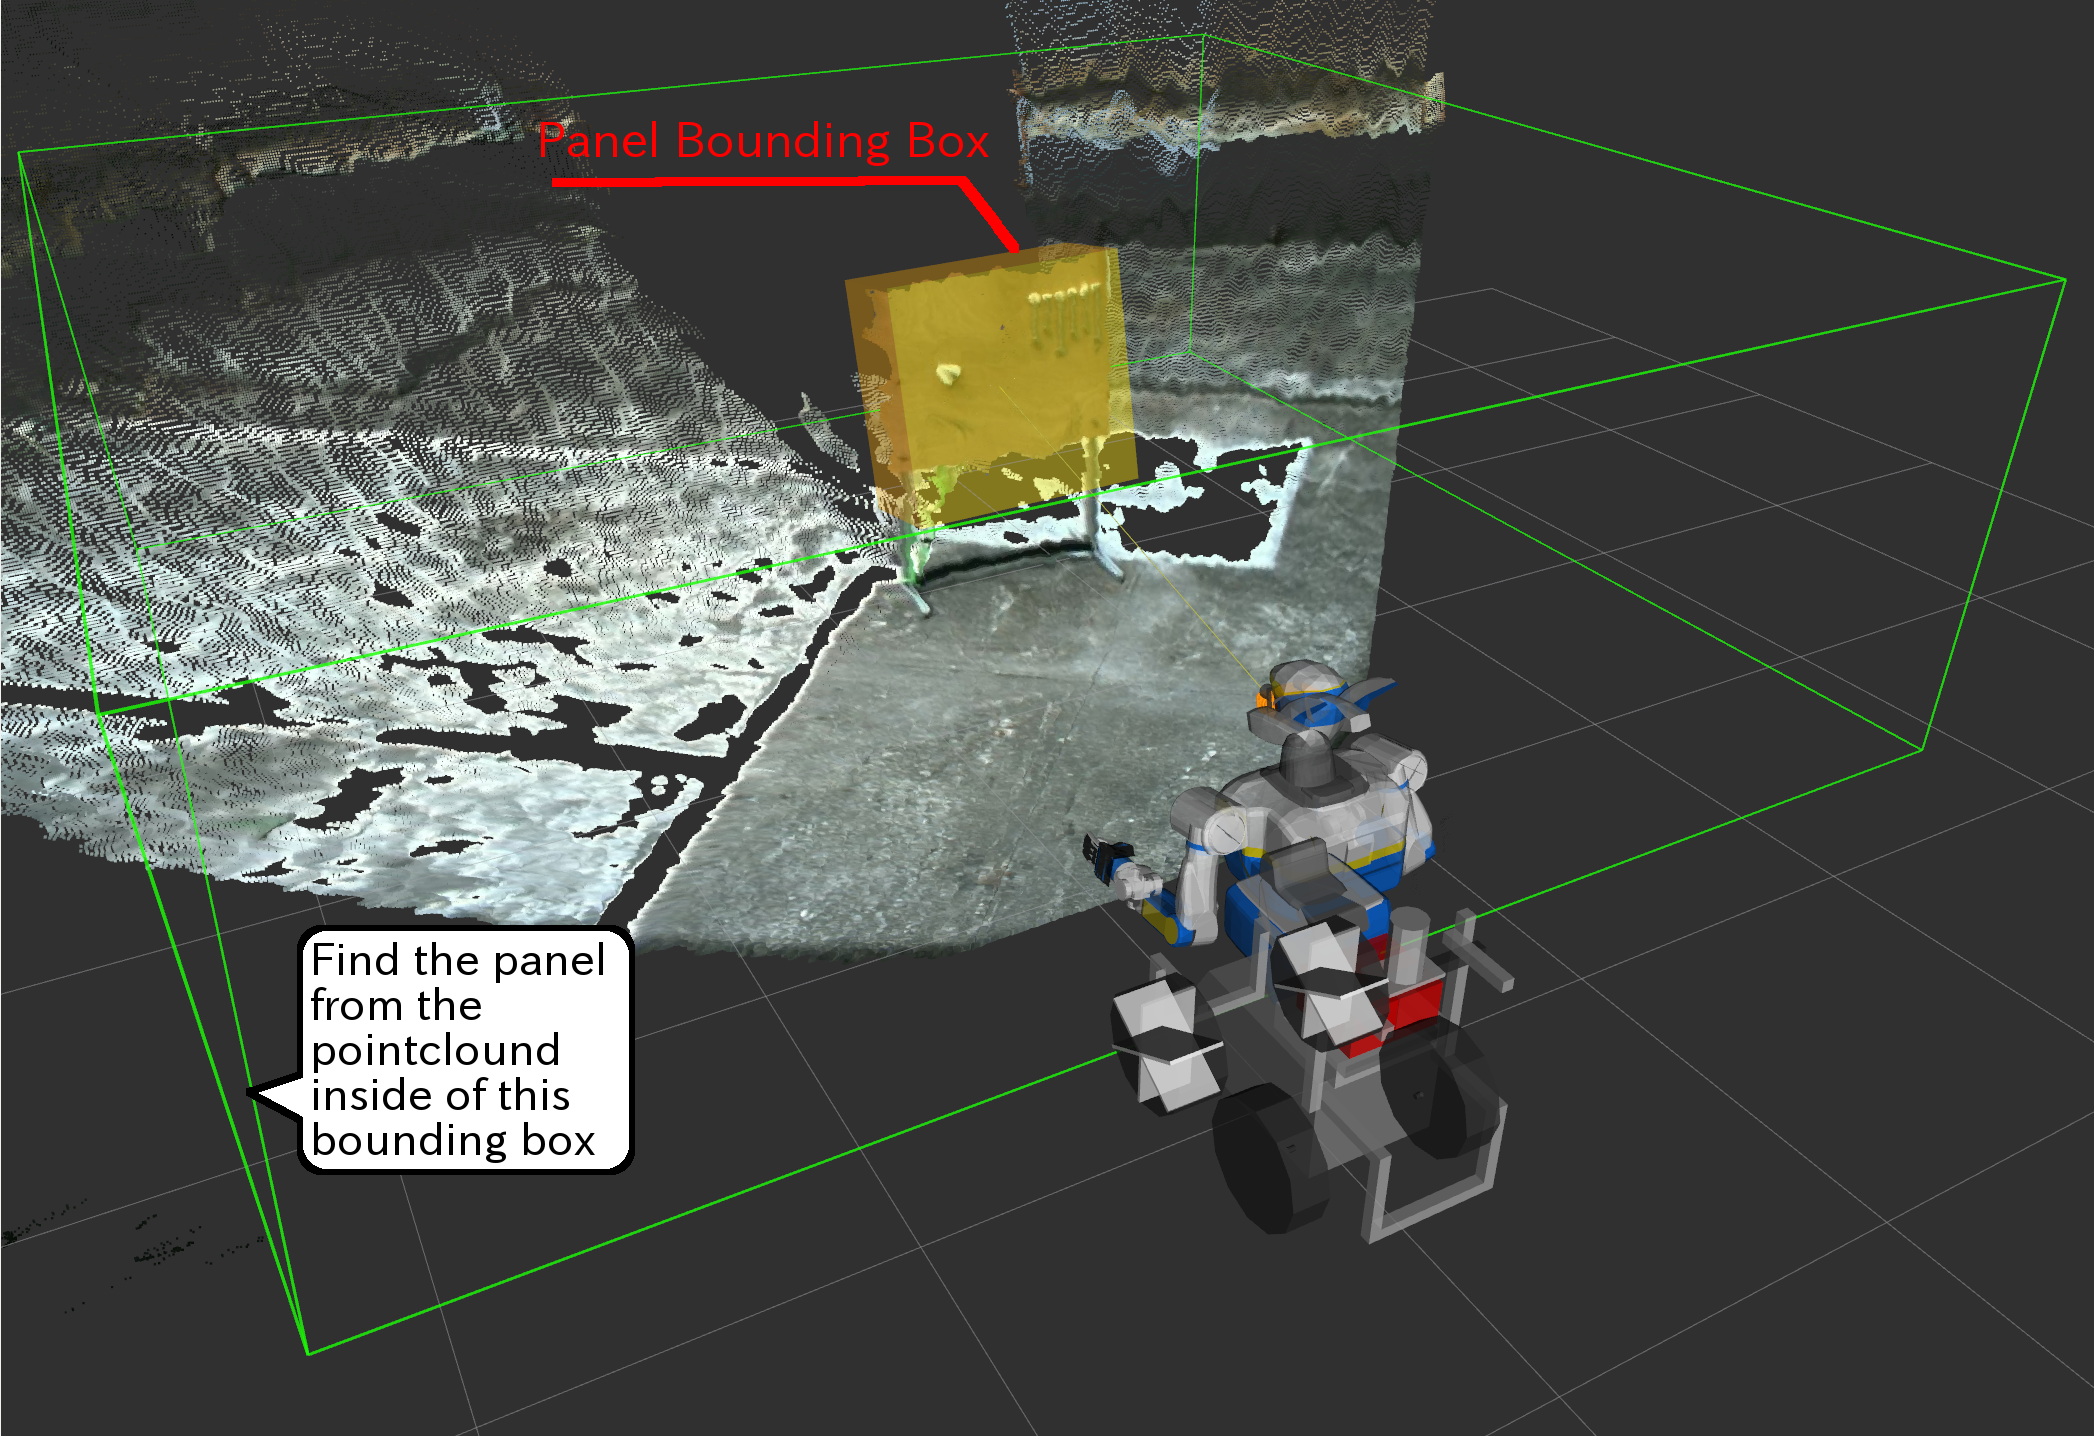
\includegraphics[width=0.80\columnwidth]{sections/task2/images/panel_detect.png}
    \caption{Panel Recognition from Pointcloud}
    \label{fig: task2_panel-recognition}
  \end{center}
\end{figure}

\subsubsection{Wrench and Valve Stem Recognition}
Previously, the wrenches and valve stem was detected on the region of
interest (ROI) which was manually annotated. From the ROI, we were
able to recognize the length of the wrenches, the position of the
wrenches and the valve stem.

% We detected the wrenches and valve stem by manually selecting an ROI
% in our previous progress report, and we were able to recognize the
% length of the wrenches, and the position of the wrenches and the valve
% stem.

We have improved our detection algorithms and made it autonomous. The
robot is now able to autonomously detect and recognize the orientation
of the panel relative to the robot frame.
% Our next target is autonomous detection and recognition of the
% orientation of the panel relative to the robot. 
This is achieved by
first fitting a plane to the 3D point clouds in front of the
robot. Next the upper right hand corner of the plane is detected and
used for calculating the orientation. The position of the wrenches and valve
stem on the panel are fixed and known in prior, hence the position and
orientations of the wrenches can easily be estimated
%determine the position and orientation 
once the panel is detected (Fig.\ref{fig: task2_object-recognition}).

We tested the detection and recognition method described above both
indoor and outdoor and confirmed the accuracy and robustness for executing this task.


\begin{figure}[htb]
  \begin{center}
    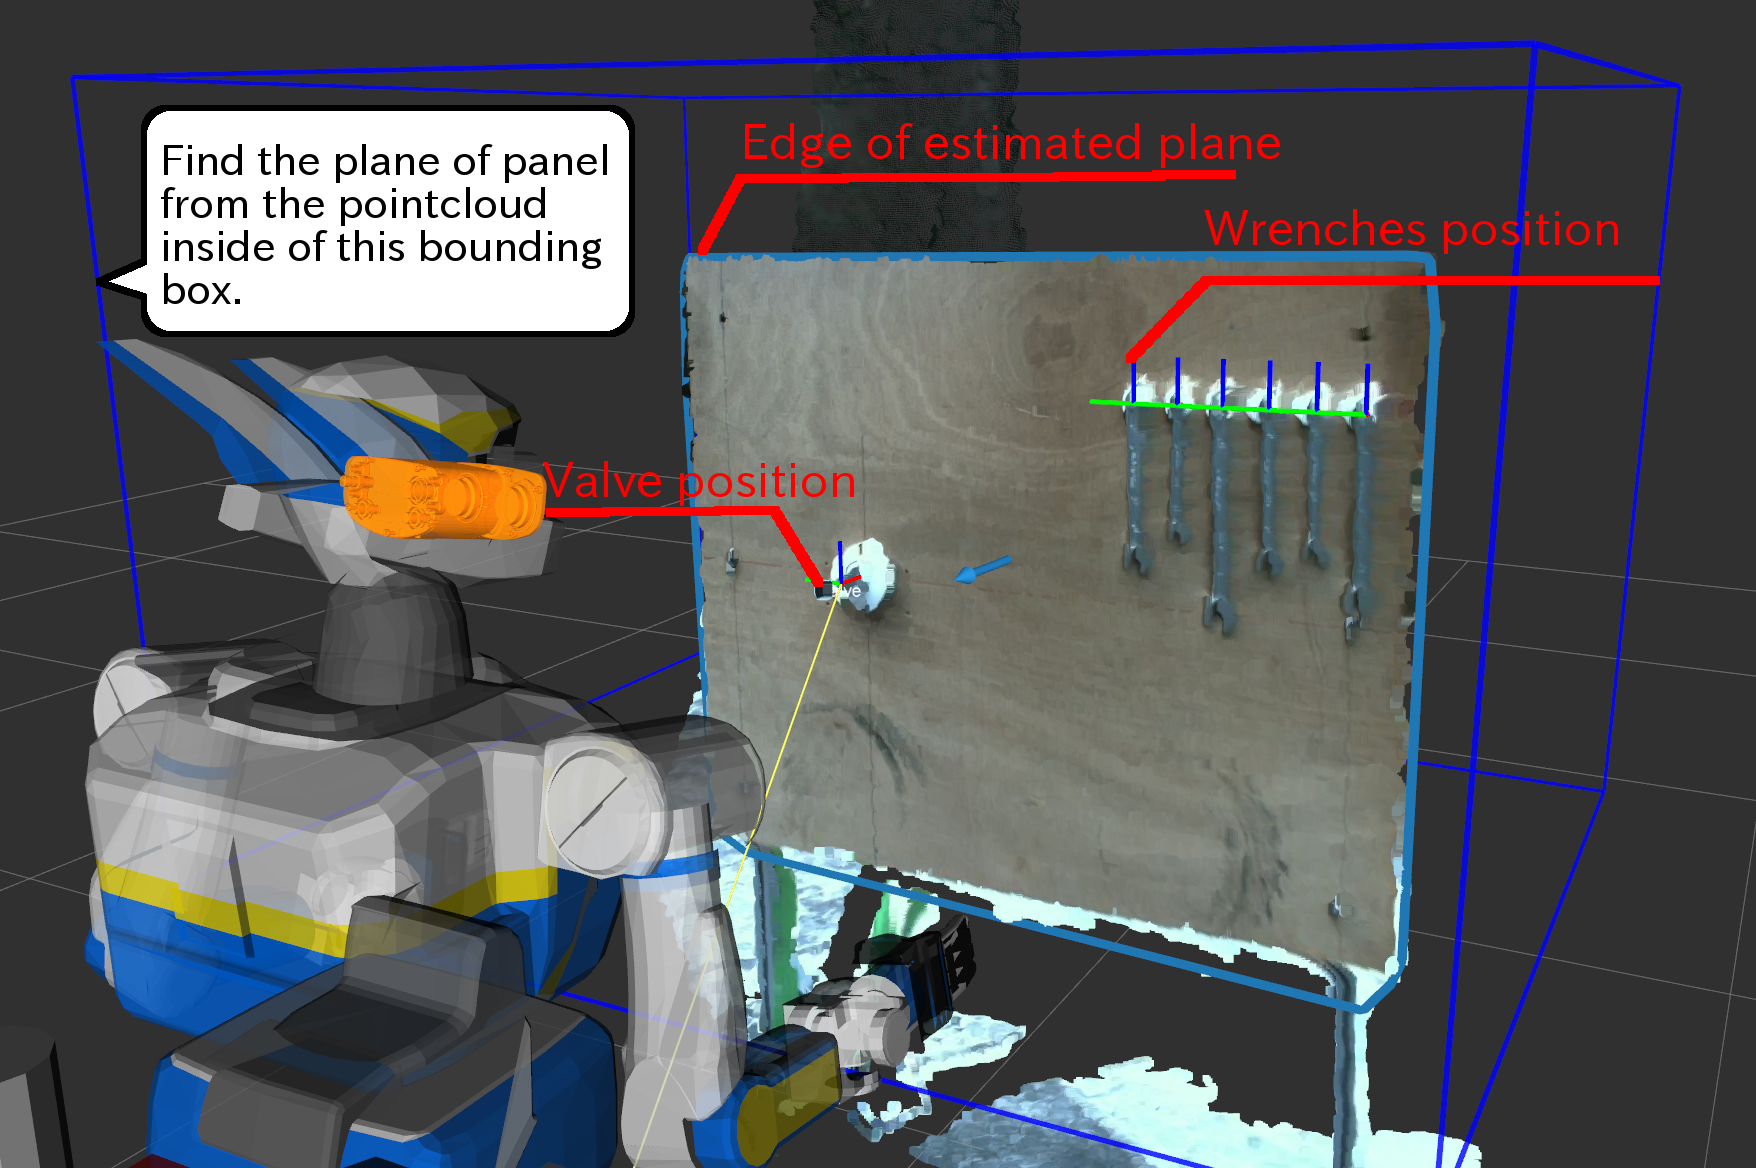
\includegraphics[width=0.80\columnwidth]{sections/task2/images/wrench_valve_recog.png}
    \caption{Wrench and Valve Stem Recognition}
    \label{fig: task2_object-recognition}
  \end{center}
\end{figure}

\subsubsection{Wrench Picking}
The robot picks the wrench by 
%We accomplished wrench picking by 
simply positioning the gripper to
the detected wrench's position in robot frame. However, the camera
resolution and calibration errors affects precise alignment for grasping.
To improve the accuracy we will use a custom made handeye camera system for visual
feedback control.

\subsubsection{Wrench Fitting and Turning}
We have accomplished wrench fitting and turning in our previous
report, and we will be using handeye visual feedback control to
improve it performance as well.

